% (c) Egor Osipov

\documentclass[a4paper,12pt]{article} % тип документа (report, book)
\usepackage[14pt]{extsizes}
\usepackage[left=2cm,right=2cm, top=2cm,bottom=2cm,bindingoffset=0cm]{geometry} % Настройки документа


%  Русский язык
\usepackage[T2A]{fontenc}			% кодировка
\usepackage[utf8]{inputenc}			% кодировка исходного текста
\usepackage[english,russian]{babel}	% локализация и переносы


% Математика
\usepackage{amsmath,amsfonts,amssymb,amsthm,mathtools} 

% Просто смайлики
\usepackage{wasysym}

%Вставка картинок
\usepackage{graphicx}
\graphicspath{./}
\DeclareGraphicsExtensions{.pdf,.png,.jpg}
\usepackage{float}

% Настройка абзацев
\usepackage{indentfirst}
%\setlength{\parindent}{5ex}
%\setlength{\parskip}{1em}

\begin{document} % начало документа

%Заговолок
\begin{titlepage}
\begin{center}
	\large{Московский физико-технический институт}\\
	\vspace{100px}
	\LARGE{Лабораторная работа № 3.1.3}\\
	\LARGE{Измерение магнитного поля земли.}\\
	\vspace{30px}
	
\includegraphics[scale = 0.3]{fakt_logo.png}\\
\end{center}

\vfill
\begin{flushright}
	\text{Осипов Егор. Б03-005}\\
	\text{06.10.2021}\\
	\text{г. Долгопрудный}
\end{flushright}
\end{titlepage}

\newpage

\tableofcontents

\newpage

\newpage

\section{Подготовка к работе.}
\subsection{Цель работы и оборудование.}

\textbf{Цель работы:} определить характеристики шарообразных неодимовых магнитов и, используя законы взаимодействия магнитных моментов с полем, измерить горизонтальную и вертикальную составляющие индукции магнитного поля Земли и магнитное наклонение.

\textbf{В работе используется:} 12 одинаковых неодимовых магнитных шариков, тонкая нить для изготовления крутильного маятника, медная проволока диаметром (0,5 – 0,6) мм, электронные весы, секундомер, измеритель магнитной индукции АТЕ-8702, штангенциркуль, брусок из немагнитного материала (25x30x60 $\text{мм}^3$ ), деревянная линейка, штатив из немагнитного материала; дополнительные неодимовые магнитные шарики (~ 20 шт.) и неодимовые магниты в форме параллелепипедов (2 шт.), набор гирь и разновесов.

\subsection{Магнитный диполь.}

Простейший магнитный диполь может быть образован витком с током или постоянным магнитом. По определению, магнитный момент $\vec{P_m}$ тонкого витка S с током I равен:

\begin{equation}\label{eq1}
\vec{P_m} = (1/c) \vec{S} = (I/c)S \vec{n}
\end{equation}

Магнитное поле точечного диполя определяется по формуле, аналогичной формуле для поля элементарного электрического диполя:

\begin{equation}\label{eq2}
\vec{B} = \frac{3(\vec{P_m} \vec{r})\vec{r}} {r^5} - \frac{\vec{P_m}}{r^3}
\end{equation}

Тогда механический момент сил, действующих в поле такого диполя:

\begin{equation}\label{eq3}
\vec{M} = \vec{P_m} \times \vec{B}
\end{equation}

Под действием вращающего момента $\vec{M}$ так, чтобы его магнитный момент выстроился вдоль вектора индукции магнитного поля. Это -- положение устойчивого равновесия: при отклонении от этого положения возникает механический момент внешних сил, возвращающий диполь к положению равновесия.

Энергия магнитного диполя в поле:

\begin{equation}\label{eq4}
W = -(\vec{P_m},\vec{B})
\end{equation}

В системе СИ размерность $[\vec{P_m}] = [W] / [B] = \text{Дж} / \text{Тл}$

В системе СГСЭ -- $[\vec{P_m}] = [W] / [B] = \text{эрг} / \text{Гс}$

Зная магнитные моменты $P_1$ и $P_2$ двух небольших постоянных магнитов, можно рассчитать силу их взаимодействия. Если магнитные моменты $P_1 = P_2 = P_m$ двух одинаковых небольших магнитов направлены вдоль соединяющей их прямой, а расстояние между ними равно r, то магниты взаимодействуют с силой:

\begin{equation}\label{eq5}
F = \frac{P_m \delta B}{\delta r} = \frac{P_m \delta (2P_m)}{r^3 \delta r} = \frac{-6 P_m^2}{r^4}
\end{equation}

\subsection{Неодиновые магнитные шары.}

В настоящей работе используются неодимовые магниты шарообразной формы.
Для нас важно то, что:

1) шары намагничены однородно;

2) вещество, из которого изготовлены магниты, является магнитожёстким материалом.

\section{Ход работы.}

\subsection{Задание 1. Метод А.}

1) Взвесим шарики на весах. Важно знать, что весы могут давать некорректные показания, если магниты класть непосредственно на платформу весов. Определим диаметр шариков.

2) Проложим между двумя магнитными шариками брусок из немагнитного материала. Подкладывая между бруском и верхним магнитиком листы бумаги (Рисунок \eqref{pic1:ref}), выяним, на каком максимальном расстоянии $r_{max}$ шарики удерживают друг друга в поле тяжести Земли.

\begin{figure}[H]
\noindent\centering{
\hspace{-0mm}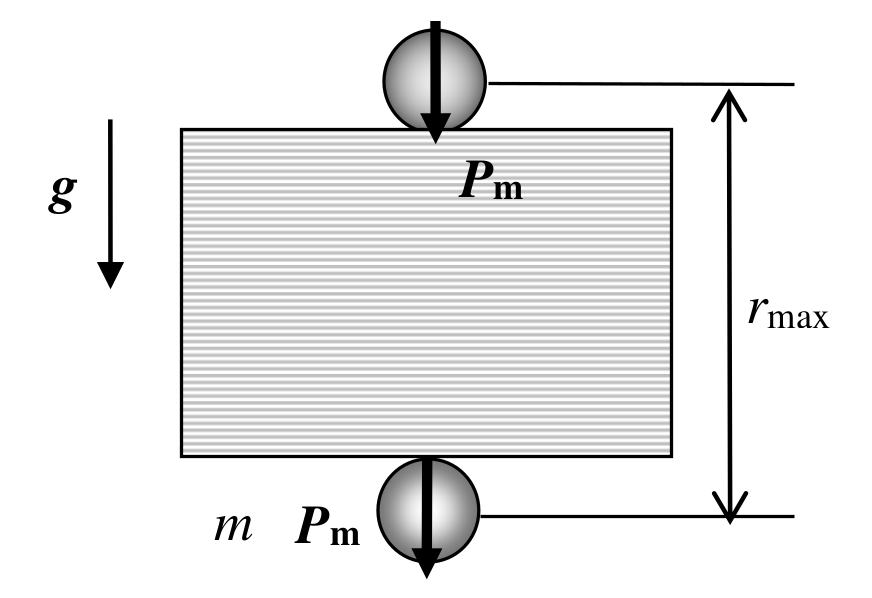
\includegraphics[scale=0.4]{pic1}
}
\caption{Определение магнитного момента шариков по силе тяжести.}
\label{pic1:ref}
\end{figure}

3) Расчитаем величину магнитного момента магнитика P m , прировняв силу притяжения двух магнитных диполей $F = 6P_m^2 /r_max^4$ к силе тяжести $F_\text{т} = mg$. Оценим погрешность измерений.

4) Рассчитайте величину намагниченности материала шариков $p_m = P_m / V$.

5) По величине магнитного момента (намагниченности) шарика, рассчитаем величину $B_p$ магнитного поля на полюсах шарика. С помощью магнетометра АТЕ-8702 измерим индукцию поля на полюсах шарика. Сравним расчетное $B_p$ значение с измеренным. При сильном расхождении результатов повторим измерения магнитного момента шарика.

6) Рассчитайте величину $B_r = 4 \pi p_m$ остаточной магнитной индукции материала, из которого изготовлен магнитный шарик. Сравните ваш результат с табличными значениями $B_r$ для соединения неодим-железо-бор.

\subsection{Задание 1. Метод Б.}

7) Используя дополнительные шарики, составим цепочку из 20-30 шариков и, с помощью неодимовых магнитов в форме параллелепипедов, подсоеденим цепочку к гире и разновесам, так, чтобы общая масса системы составила ~ 500 г (Рис \eqref{pic2:ref} (б)). Добавляя или удаляя шарики (шарики можно примагничивать непосредственно к гире), подберем минимальный вес F системы цепочки с гирей, при котором она отрывается от верхнего шарика.

\begin{figure}[H]
\noindent\centering{
\hspace{-0mm}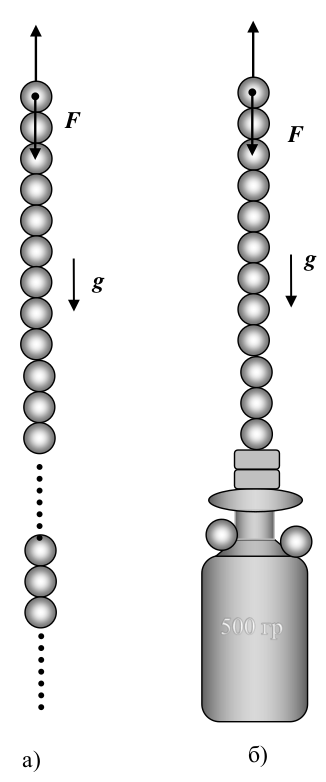
\includegraphics[scale=0.4]{pic2}
}
\caption{Определение магнитного момента шариков по силе сцепления.}
\label{pic2:ref}
\end{figure}

8) С помощью весов определим вес F оторвавшейся цепочки с гирей.

9) По формуле $F_0 = F/1.08$ определим силу сцепления двух шаров.

10) Из формулы $F_0 = 6P_m^2 /d^4$ определим магнитный момент шарика $P_m$. Оценим погрешность результата.

11) Рассчитаем величину поля на полюсах и сравним расчетное значение с измеренным магнетометром АТЕ-8702.

12) Сравним значения магнитных моментов, полученные методом A и методом B.

13) Окончательный результат измерений $P_m$ занесем в Таблицу (------).

\subsection{Задание 2. Определение горизонтальной составляющей магнитного поля Земли.}

Схема установки, предназначенной для измерения горизонтальной составляющей поля Земли, показана на Рисунке \eqref{pic3:ref}. Это крутильный маятник в виде магнитной <<стрелки>> закреплённой на тонкой нити. Магнитная <<стрелка>> собирается из $n = 3..12$ магнитных шариков и подвешивается в горизонтальном положении с помощью $\bigwedge$-образного подвеса. Маятник совершает крутильные колебания вокруг вертикальной оси, проходящей через центр масс <<стрелки>>. Для крепления нити в работе используется штатив, изготовленный из немагнитного материала.

\begin{figure}[H]
\noindent\centering{
\hspace{-0mm}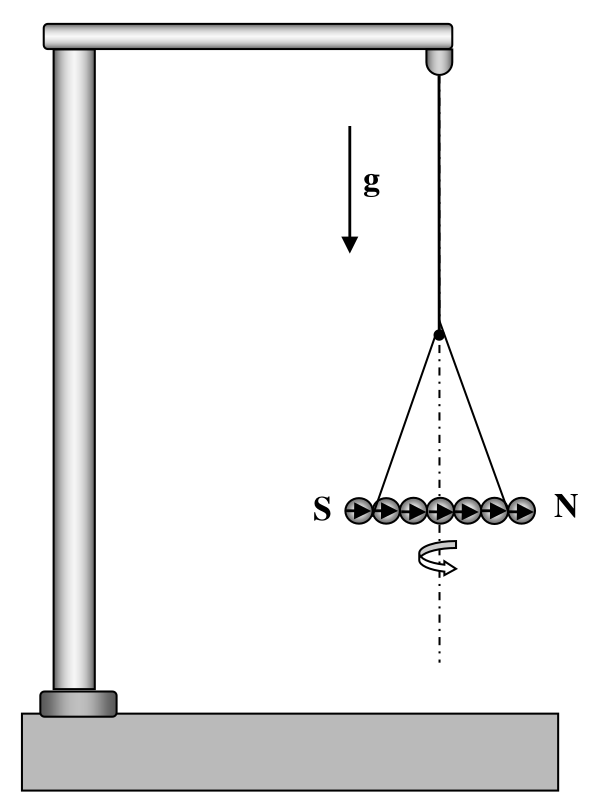
\includegraphics[scale=0.4]{pic3}
}
\caption{Схема установки для определения горизонтальной составляющей магнитного поля Земли.}
\label{pic3:ref}
\end{figure}

14) Соберем крутильный маятник и, используя $\bigwedge$-образного подвес, установим <<магнитную стрелку>> из 12 магнитных шариков в горизонтальном положении (юстировка системы).

15) Возбудим крутильные колебания маятника вокруг вертикальной оси и определим их период. Оценим влияние упругости нити на период колебаний, возбудив крутильные колебания <<стрелки>>, свёрнутой в кольцо (очевидно, что магнитный момент такого кольцеобразного маятника равен нулю) (Рисунок \eqref{pic4:ref}). Покажем, что упругость нити при расчете периода колебаний можно не учитывать.

\begin{figure}[H]
\noindent\centering{
\hspace{-0mm}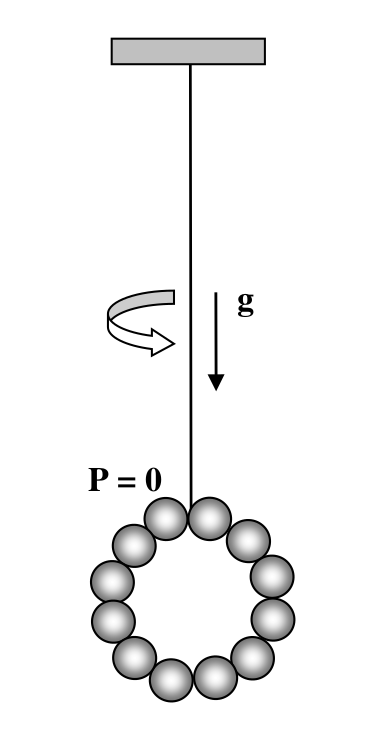
\includegraphics[scale=0.4]{pic4}
}
\caption{Магнитная <<стрелка>>, свернутая в кольцо.}
\label{pic4:ref}
\end{figure}

16) Исследуем зависимость периода T крутильных колебаний <<стрелки>> от количества магнитных шариков n, составляющих <<стрелку>>. Измерения проведем для значений $n = 3..12$. (Не забудем для каждого значения n юстировать систему, выставляя перед каждым измерением <<стрелк>> горизонтально).

17) Построим график экспериментальной зависимости T(n).

18) Аппроксимируем экспериментальную мость T(n) прямой T = kn.

19) По значению углового коэффициента k рассчитаем величину горизонтальной составляющей магнитного поля Земли по формуле:

\begin{equation}\label{6}
B_h = \pi^2md^2 / 3k^2P_m
\end{equation}

Оценим погрешность измерений.

\subsection{Задание 3. Определение вертикальной составляющей магнитного поля Земли.}

20) Изготовим магнитную <<стрелку>> из n = 10 шариков и подвесим её за середину с помощью нити на штативе (Рисунок \eqref{pic5:ref}, а)

\begin{figure}[H]
\noindent\centering{
\hspace{-0mm}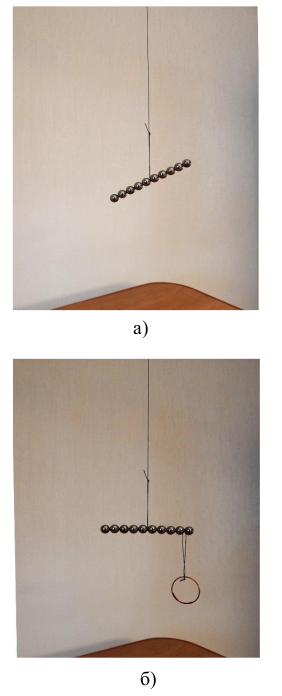
\includegraphics[scale=0.7]{pic5}
}
\caption{Определение вертикальной составляющей магнитного поля.}
\label{pic5:ref}
\end{figure}

21) Определим механический момент сил, действующий со стороны магнитного поля Земли на горизонтально расположенную магнитную <<стрелку>>. Для этого, с помощью одного или нескольких кусочков проволоки, уравновесим <<стрелку>> в горизонтальном положении (Рисунок \eqref{pic5:ref}, б).

22) С помощью весов определите массу уравновешивающего груза $m_\text{гр}$.

23) Из условия равновесия рассчитаем механический момент сил M, действующих на горизонтальную <<стрелку>> со стороны поля Земли. Измерения момента сил M(n) проведем для чётных значений n = 4, 6, 8, 10, 12 (у таких <<стрелок>> есть <<хорошая серединка>> для подвешивания на нити).

24) Построим график экспериментальной зависимости M = M(n).

25) Аппроксимируем экспериментальную зависимость M(n) прямой линией M = An.

26) По значению углового коэффициента A зависимости M = An рассчитайте величину $B_{\nu}$ вертикальной составляющей магнитного поля Земли $B_{\nu} = A/P_m$. Оцените погрешность измерений $B_{\nu}$.

27) Используя результаты измерений $B_{\nu}$ и $B_h$, определим магнитное наклонение $\beta$ и полную величину индукции магнитного поля Земли на широте Долгопрудного. Сравним полученное значение наклонения с расчетным, полученным в предположении, что поле Земли соответствует полю однородного намагниченного вдоль оси вращения шара. Широту Долгопрудного возьмем равной $\phi = 56\deg$ с.ш. (северной широты). Оценим также полный магнитный момент $P_\text{З}$ Земли.

28) Сравним полученные в работе результаты с современными справочными данными параметров магнитного поля Земли в Московском регионе.

\section{Результаты и обработка.}

\subsection{Задание 1.}

Способ А:\\
$m_0 = 0.483 \pm 0.001$г, $r_\text{max} = 16.00 \pm 0.05$мм.\\
$F = \frac{6P_m^2}{r_{max^4}} = m_0g$\\
$P_m = 7.190 \pm 0.047 \cdot 10^{-6}\;$\\
$\rho_m = \frac{P_m}{V} = 141.16 \pm 0.92$ Тл/м$^3$\\
$B_p = 1182.5\pm7.7,\;\;\;B_r = 1773\pm11$\\

Способ В:\\
M = 258.36г
$F_0 = 2.34\;$Н\\
$P_m = 13.20 \pm 1.34 \cdot 10^{-6}\;$\\
$B_p = 16\frac{P_m}{d_0^3} = (1.808 \pm 0.183) \times 10^{3}\;$ Тл


\begin{table}[H]
\caption{\label{tab:canonsummary} Итог}
\begin{center}
\begin{tabular}{|c|c|}
\hline
$P_m(A)$ & $P_m(B)$\\
\hline
$7.19 \pm 0.47 \cdot 10^{-6}$ & $13.20 \pm 1.34 \cdot 10^{-6}$\\
\hline
\end{tabular}
\end{center}
\label{table1:ref}
\end{table}

Далее будем считать $P_m = 9.52 * 10^{-6}$. 

\subsection{Задание 2.}

\begin{table}[H]
\caption{\label{tab:canonsummary} Зависимость периода колебаний от количества шариков.}
\begin{center}
\begin{tabular}{|c|c|c|c|}
\hline
n & $n_0$ & t (сек) & T (сек)\\
\hline
12 & 30 & 92.8 & 3.09\\
\hline
11 & 30 & 87.6 & 2.92\\
\hline
10 & 30 & 74.5 & 2.48\\
\hline
9 & 30 & 70.2 & 2.34\\
\hline
8 & 30 & 61.1 & 2.04\\
\hline
7 & 30 & 55.8 & 1.86\\
\hline
6 & 33 & 53.3 & 1.62\\
\hline
5 & 33 & 43.6 & 1.32\\
\hline
4 & 30 & 32.2 & 1.07\\
\hline
3 & 30 & 25.3 & 0.84\\
\hline
\end{tabular}
\end{center}
\label{table1:ref}
\end{table}

\begin{equation}\label{eq11}
B_h = \frac{\pi^2 m d_0^2}{3 k^2 P_m} = 56 \pm 7\text{мкТл}
\end{equation}

\begin{figure}[H]
\noindent\centering{
\hspace{-0mm}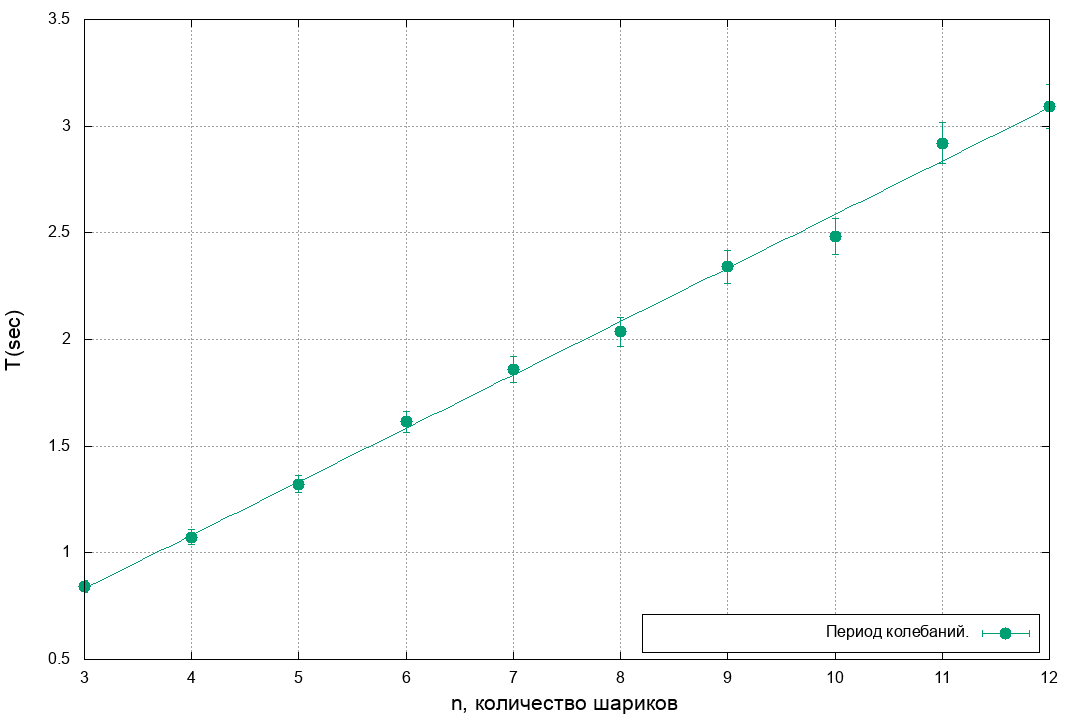
\includegraphics[scale=0.5]{1st_plot}
}
\caption{Зависимость периода колебаний от количества шариков.}
\label{pic4:ref}
\end{figure}

\subsection{Задание 3.}

\begin{table}[H]
\caption{\label{tab:canonsummary} Зависимсоть момента от количества шариков.}
\begin{center}
\begin{tabular}{|c|c|}
\hline
n & $M \cdot 10^{-6}$ (Н/м)\\
\hline
10 & 3.13\\
\hline
8 & 3.06\\
\hline
6 & 1.38\\
\hline
4 & 1.15\\
\hline
\end{tabular}
\end{center}
\label{table1:ref}
\end{table}

\begin{figure}[H]
\noindent\centering{
\hspace{-0mm}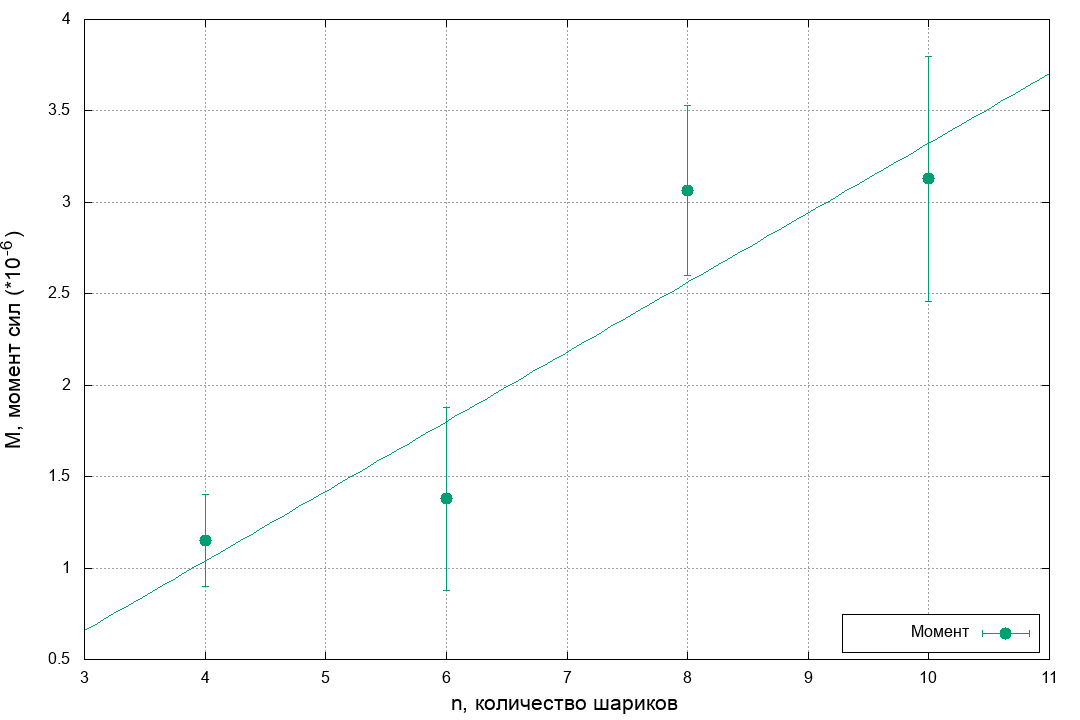
\includegraphics[scale=0.5]{2nd_plot}
}
\caption{Зависимость момента сил от количества шариков.}
\label{pic4:ref}
\end{figure}

$k = 3.18 \pm 0.70 \cdot 10^{-7}$\\
$$B_\upsilon = \frac{k}{P_m} = 0.033 \pm 0.011\;\text{мкТл}$$

\section{Вывод}

Магнитное поле Земли составило по оценкам этой работы $\beta = 56\pm 7\;$мкТл.

\end{document}